% $Id: notes_2021.tex,v 1.2 2021/10/31 03:19:57 brandenb Exp $
%\documentclass{article}
\documentclass[twocolumn]{article}
\setlength{\textwidth}{170mm}
\setlength{\oddsidemargin}{-0mm}
\setlength{\textheight}{260mm}
\setlength{\topmargin}{-28mm}
\usepackage{graphicx,natbib}
\usepackage{bm,html,url}
\graphicspath{{./fig/}{./png/}}
\input macros
\title{Timing results for Dardel}
\author{Axel Brandenburg}
\date{\today,~ $ $Revision: 1.2 $ $}
\begin{document}
\maketitle

\section{Code and test case}

For all tests, the {\sc Pencil Code} was used.
It is publicly available on \url{http://github.com/pencil-code},
where also detailed documentation is available.
The code uses explicit sixth order finite differences.
The time step is third-order.
In this sample, we run isothermal magnetohydrodynamics
in a periodic domain\footnote{A sample run directory is available on
\url{https://github.com/pencil-code/pencil-code/tree/master/doc/timings/N4096_32x32x32}}.

\begin{table}[h!]\caption{
Dardel timings
}\vspace{12pt}\centerline{\begin{tabular}{rcccc}
proc & $\displaystyle\frac{{\mu\rm s}}{\rm pt\;\;step}$ & resol. & layout & comp. \\
\hline
 128 & 6.346E-03 &$256^3$ & 4x4x8 & Cray\\
 256 & 3.215E-03 &$256^3$ & 4x8x8 & Cray\\
 512 & 1.857E-03 &$256^3$ & 8x8x8 & Cray\\
1024 & 1.505E-03 &$256^3$ & 8x8x16 & Cray\\
2048 & 1.884E-03 &$256^3$ & 8x16x16 & Cray\\
\hline
 512 & 1.571E-03 &$512^3$ & 8x8x8\\
1024 & 1.102E-03 &$512^3$ & 8x8x16b\\
2048 & 5.508E-04 &$512^3$ & 8x16x16\\
4096 & 7.461E-04 &$512^3$ & 16x16x16\\
 512 & 1.568E-03 &$512^3$ & 8x8x8 & gnu\\
1024 & 9.260E-04 &$512^3$ & 8x8x16 & gnu\\
2048 & 5.550E-04 &$512^3$ & 8x16x16 & gnu\\
4096 & 7.702E-04 &$512^3$ & 16x16x16 & gnu\\
\hline
 4096 & 2.093E-04 &$1024^3$ & 16x16x16 & Cray\\
 8192 & 1.215E-04 &$1024^3$ & 16x16x32 & Cray\\
16384 & 8.536E-05 &$1024^3$ & 16x32x32 & Cray\\
 4096 & 2.754E-04 &$1024^3$ & 16x16x16 & gnu\\
 8192 & 1.194E-04 &$1024^3$ & 16x16x32 & gnu\\
16384 & 6.046E-05 &$1024^3$ & 16x32x32 & gnu\\
32768 & 3.953E-05 &$1024^3$ & 32x32x32 & gnu\\
\hline
 2048 & 3.416E-04 &$2048^3$ & 8x16x16 \\
 4096 & 1.859E-04 &$2048^3$ & 8x16x32 \\
 4096 & 1.674E-04 &$2048^3$ & 16x16x16 \\
 8192 & 9.271E-05 &$2048^3$ & 16x16x32 \\
16384 & 6.853E-05 &$2048^3$ & 16x32x32 \\
32768 & 2.909E-05 &$2048^3$ & 32x32x32 \\
\hline
 8192 & 8.588E-05 &$4096^3$ & 16x16x32 \\
16384 & 4.368E-05 &$4096^3$ & 16x32x32 \\
32768 & 3.153E-05 &$4096^3$ & 32x32x32 \\
\label{Tsummary}\end{tabular}}\end{table}

\section{Running the code}

To run the code, get one of the sample run directories, e.g.,
\url{https://github.com/pencil-code/pencil-code/tree/master/doc/timings/N4096_32x32x32}.
The relevant file to be changed is \url{src/cparam.local}
\scriptsize
\begin{verbatim}
ncpus=32768,nprocx=32,nprocy=32,nprocz=ncpus/(nprocx*nprocy)
nxgrid=4096,nygrid=nxgrid,nzgrid=nxgrid
\end{verbatim}
\normalsize
In particular, the values of ncpus, nprocx, nprocy, and nxgrid.
Once they are chosen, say make, and submit
start\_run.csh.

\begin{figure}[h!]\begin{center}
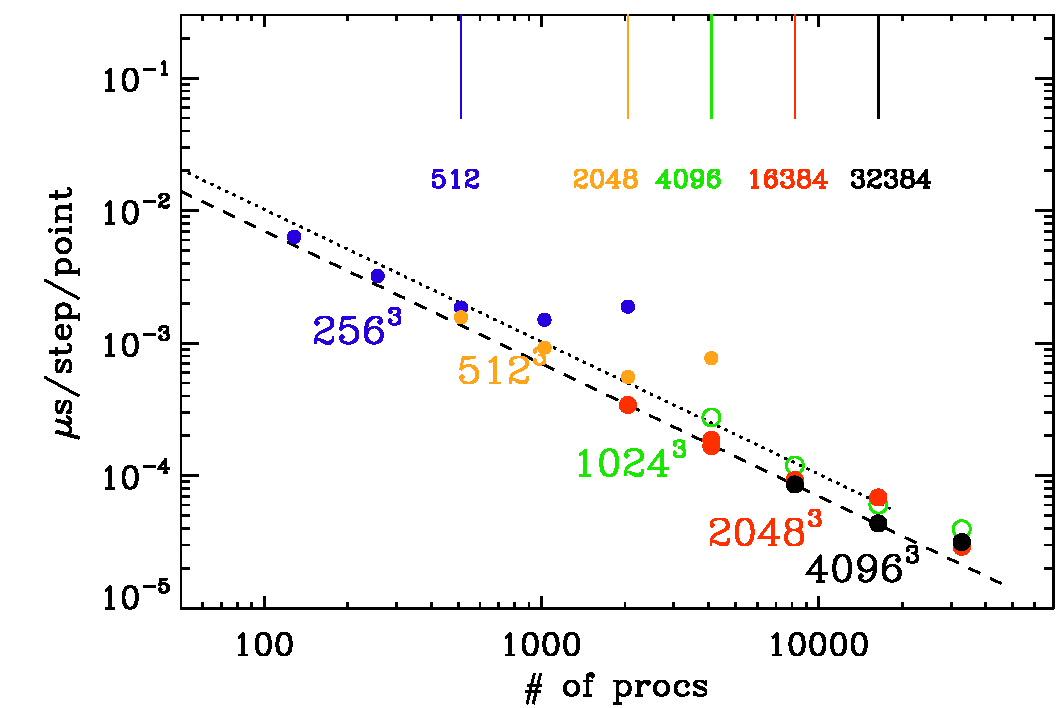
\includegraphics[width=\columnwidth]{pdardel_strong}
\end{center}\caption[]{
Strong scaling on Dardel.
The dotted and dashed lines corresponds to
$1.02\mu{\rm s}/{\rm proc}/{\rm step}/{\rm point}$ and
$0.70\mu{\rm s}/{\rm proc}/{\rm step}/{\rm point}$, respectively.

}\label{pdardel_strong}\end{figure}

\section{Dardel results}

On Dardel, strong scaling tests have been performed
for five mesh sizes.
The time per time step and mesh point is given for
different processor numbers and layouts.
Generally, it is advantageous to minimize the
processor surface area, and to keep the number
of processors in the $x$ direction small.

{\em Comments}.~
Performancewise, Cray with O2 optimization is equivalent to gnu with O3.
While gnu-O3 is able to handle memory or whatever compiler problems much
better, it is otherwise not better than Cray-O2, and often some 10--20\%
slows, but this is within the measurement accuracy.

%r e f
%\begin{thebibliography}{}

%\bibitem[Biskamp \& M\"uller(1999)]{BM99}
%Biskamp, D., \& M\"uller, W.-C.\yprl{1999}{83}{2195}

%\end{thebibliography}

\vfill\bigskip\noindent\tiny\begin{verbatim}
$Header: /var/cvs/brandenb/tex/pencil-code/performance/notes_2021.tex,v 1.2 2021/10/31 03:19:57 brandenb Exp $
\end{verbatim}

\end{document}
